\documentclass[a4paper]{article}
\usepackage[utf8]{inputenc}
%\usepackage[latin1]{inputenc}
\usepackage[T1]{fontenc}
\usepackage[brazil]{babel}
%\usepackage{ntheorem}
\usepackage[pdftex]{graphicx}
%\usepackage{subfigure}
\usepackage[top=3cm, bottom=2cm, left=3cm, right=2cm]{geometry} 
\usepackage{enumerate} 
\usepackage{amsmath}
\usepackage{float}
\usepackage{url}
\usepackage{caption}
\usepackage{subcaption}
\usepackage{graphicx}
\usepackage{listings}
%\usepackage[space]{grffile}

%\usepackage{etoolbox}
%\makeatletter
%\patchcmd{\Ginclude@eps}{"#1"}{#1}{ }{}
%\makeatother

\newcommand{\BigO}[1]{\ensuremath{\operatorname{O}\bigl(#1\bigr)}}

\begin{document}

%\bibliographystyle{alpha} % Choose Phys. Rev. style for bibliography


\title{Trabalho Prático III - Recuperação de Informação}
\author{Prof. Nivio Ziviani e Prof. Berthier Ribeiro-Neto \\ \\ Evelin Carvalho Freire de Amorim}
%\date{\today}

\maketitle

\tableofcontents 

\section{Introdução}

Fazer consultar em máquinas de busca é um hábito rotineiro para pessoas no mundo todo. 
Os resultados das consultas feitas por diversas pessoas são listagens ordenadas de 
páginas da \emph{web}. A ordenação empregada pela máquina de busca é fundamental 
para motivar o uso pelas pessoas. Assim muitas pesquisas procuram encontrar uma fórmula 
eficaz de comparar páginas a fim de determinar qual é a página mais relevante.

As fórmulas desenvolvidas para comparar páginas atribuem uma pontuação para páginas 
de acordo com o conteúdo dela. Contudo nem sempre apenas o conteúdo consegue representar 
a relevância em relação a consulta. Por exemplo, consultas que procuram por um 
\emph{website} são consultas cuja a url do \emph{website} é mais relevante que o 
conteúdo do \emph{website}. 

Uma forma de representar a relevância de uma página, além do conteúdo textual da mesma, 
é através de referências de outras páginas para ela. A intuição desta ideia é que páginas 
relevantes são referenciadas por páginas relevantes. Page, Brin, Motwani e Winograd
propuseram esta ideia em 1998 e chamaram a estratégia de \emph{Pagerank}~\cite{page1999pagerank}. 
Utilizando fórmulas baseadas em conteúdo e pagerank, Page e Brin criaram uma máquina de 
busca cujo resultado foi superior aos resultados da época. 

Este trabalho procura implementar um sistema que as consultas se baseiam em 
características textuais e também no cálculo do pagerank proposto originalmente. Este 
relatório descreve os detalhes da estratégia escolhida e também dos resultados obtidos.


\section{Metodologia}

O sistema de busca engloba duas partes: o índice e 
o cálcula da relevância de documentos. O índice, embora já descrito no 
relatório do trabalho prático 1, foi modificado e será brevemente 
resumido na Subseção \ref{sec:implementacao}.

Os \emph{rankings} implementados no trabalho serão brevemente explicados 
na seção \ref{sec:ranking}. A fórmula do \emph{pagerank} será explicada 
na subseção \ref{sec:pagerank}.

Além das modificações do índice alguns detalhes de implementação também serão 
relatados na Seção \ref{sec:implementacao}.

\subsection{Medidas de \emph{Ranking}}\label{sec:ranking}

Os dois rankings mais populares em recuperação de informação são BM25 e Vetorial. 
A medida BM25 foi desenvolvida com base em três principios: frequência inversa 
do documento, frequência do termo e normalização do documento. A  Fórmula \ref{eq:rankingprob} é 
a equação do BM25, onde  $d_j$ é um documento, $q$ é a consulta, $k_i$ é um termo, 
$N$ é o número de documentos na coleção e $n_i$ é o número de termos onde 
$k_i$ ocorre.


\begin{equation}
    sim(d_j,q) \sim \sum_{k_i \in q \wedge k_i \in d_j} \log{\left(\frac{N-n_i+0.5}{n_i+0.5}\right)}
    \label{eq:rankingprob}
\end{equation}

No entanto como a Fómula \ref{eq:rankingprob} possui alguns problemas, como 
a não normalização do tamanho de documentos. Para tentar resolver este problema 
a Fórmula \ref{eq:bm25} foi proposta. Veja que 
a Fórmula \ref{eq:combinacao}, que está contida na formulação do BM25, nada mais é 
que uma combinação de valores relacionados a frequência do termo.

\begin{equation}
    \mathcal{B}_{i,j} = \frac{(K_1 +1)f_{i,j}}{K_1 \left[ (1-b) + b\frac{len(d_j)}{avg\_doclen}\right] + f_{i,j}}
    \label{eq:combinacao}
\end{equation}

\begin{equation}
    sim_{BM25}(d_j,q) \sim \sum_{k_i[q,d_j]} \mathcal{B} \times \log{\left(\frac{N-n_i+0.5}{n_i+0.5}\right)}
    \label{eq:bm25}
\end{equation}

Mais detalhes sobre o BM25 podem ser vistos em \cite{Baeza1999}.

A fórmula do ranking vetorial faz um produto interno entre o vetor de pesos do documento e 
da consulta. Cada componente do vetor de pesos do documento é descrito pela Fórmula \ref{eq:pesodoc}. 
As componentes do vetor da consulta são similares a do documento, como podemos 
constatar pela Fórmula \ref{eq:pesoconsulta}. Contudo a frequência $f_{i,j}$ do i-ésimo 
termo na consulta quase sempre 
é 1 e assim o valor de $\log f_{i,j}$ é 0 e a fórmula para a consulta pode 
ser representada muitas vezes por apenas por $\log{\frac{N}{n_i}}$.

\begin{equation}
    w_{i,q} = (1+\log{f_{i,q}}) \times \log{\frac{N}{n_i}}
    \label{eq:pesoconsulta}
\end{equation}

\begin{equation}
    w_{i,j} = (1+\log{f_{i,j}}) \times \log{\frac{N}{n_i}}
    \label{eq:pesodoc}
\end{equation}

Após calcular as componentes do documento e da consulta utilizamos a Fórmula \ref{eq:vetorial} para 
computarmos a similaridade entre o documento e a consulta.

\begin{equation}
    sim(d_j,q) = \frac{\sum^t_{i=1} w_{i,j} \times w_{i,q}}{\sqrt{\sum^t_{i=1} w_{i,j}^2}\times \sqrt{\sum^t_{i=1}w^2_{i,q}}}
    \label{eq:vetorial}
\end{equation}

Exemplos com a Fórmula \ref{eq:vetorial} podem ser visto em \cite{Baeza1999}.

\subsection{Pagerank}\label{sec:pagerank}

O PageRank foi proposto em 1998 em um relatório técnico \cite{page1999pagerank}. 
Para compreender o conceito de Pagerank, devemos considerar a web como um grafo cujos 
nós são as páginas e arestas direcionadas são os links de uma página para outra. A partir 
desta estrutura assumimos que quando uma página A aponta para uma página B, então é como se A votasse em B. 
Com esta suposição, consideramos que páginas que são muito votadas são páginas mais 
``importantes'' que páginas pouco votadas.

A ideia do Pagerank é formalizada pela Fórmula \ref{eq:eqpagerank}, onde $u$ é 
uma página web, $F_u$ 
é o conjunto de páginas que $u$ aponta, $B_u$ é o conjunto de páginas que apontam 
para $u$, $c$ é um fator de normalização e $N_u$ é o número de elementos em $F_u$.

\begin{equation}
    PR(u) = c \sum_{v \in B_u}\frac{PR(v)}{N_v}
    \label{eq:eqpagerank}
\end{equation}


\subsection{Implementação}\label{sec:implementacao}

Considerando os módulos anteriormente implementados não foram modificados, 
a descrição da implementação foi dividida apenas em dois módulos: 
Índice e \emph{Ranking}. 

\subsubsection{Índice}

%== Indice ==
%como funciona o indice resumidamente

%explicar modificacoes: inclusao de anchor text

%como eh computado o pagerank, emq uais funcoes? quanto ocupa de memoria?
%quantas iteracoes sao assumidas? (50)

%Como o oneurl normaliza a url?
A implementação do sistema de índice está como na arquitetura 
da Figura . Portanto o funcionamento geral é similar ao do 
sistema entregue no trabalho prático 1. 

\begin{figure}[H]
    \centering
    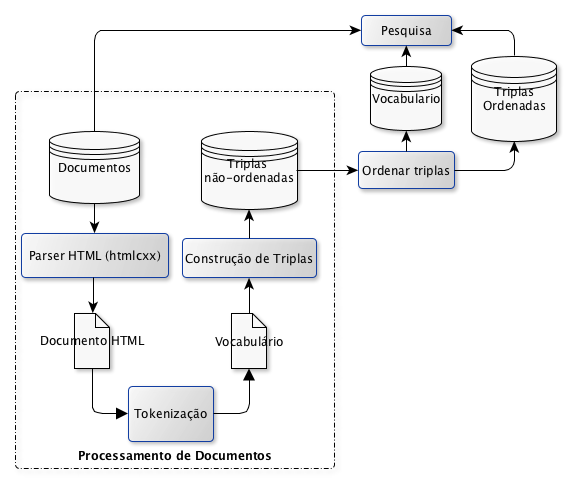
\includegraphics[scale=0.5]{arquiteturaindex.png}
    \label{pic:arquiteturaindice}
    \caption{Arquitetura do Índice}
\end{figure}

Um dos requisitos do trabalho prático atual foi a inclusão de 
texto âncora de forma a enriquecer o índice. No entanto, por falta de 
entendimento, no trabalho prático 1 o texto âncora já era indexado. Assim 
foi feito apenas um teste com um índice sem o vocabulário do texto âncora e com 
o vocabulário do texto âncora.

Uma melhoria possível no sistema é construir um índice separado para
o texto âncora. De acordo com Zaragoza et. al 
\cite{zaragoza2004microsoft}, dando um peso diferenciado para título, corpo 
e texto âncora de uma página, a performance do ranking é superior quando 
todos estes campos possuem o mesmo peso.

O sistema de indexação também foi modificado para incluir um sistema 
de indexação de \emph{links}. Esta indexação foi feita utilizando 
uma tabela \emph{hash} nativa do C++ chamada \texttt{unordered\_map}\cite{cplusplus}. 
Esta biblioteca foi escolhida em razão da sua rapidez no tempo de resposta 
na busca. De acordo com a referência gasta em média \BigO{1} para buscar 
na tabela um elemento e no pior caso \BigO{n}.

Nesta tabela de links foi feita a reserva de memória para cada link conforme 
necessidade. A tabela também é construída apenas com links da própria base, 
se houver links apontados por páginas da base, mas cujos documentos não 
existem na base, eles serão apenas ignorados nesta estratégia. 
O preenchimento desta tabela é feita na classe \texttt{Colecao}, na 
função \texttt{ler\_arvore\_dom}. A seguir o trecho de código no 
arquivo colecao.cpp em que a tabela de links é preenchida.

\texttt{//verificar se estamos dentro de uma tag de link }

\texttt{if (tag == ``a'' || tag == ``A'')\{}

\texttt{//esta variavel indica inicio de um trecho do html em que estamos dentro de um link}

\hspace{0.5cm}\texttt{islink = true;}

\hspace{0.5cm}\texttt{it->parseAttributes();}

\hspace{0.5cm}\texttt{string link\_href;}

\hspace{0.5cm}\texttt{//MAIOR\_LINK eh uma constante inicializada com 800}

\hspace{0.5cm}\texttt{link\_href.reserve(MAIOR\_LINK+2);}

\hspace{0.5cm}\texttt{link\_href = curl.CNormalize(it->attribute(``href'').second);}

\hspace{0.5cm}\texttt{if (link\_href.size(>0)\{}

\hspace{1.0cm}\texttt{//copiando os 800 primeiros caracteres}

\hspace{1.0cm}\texttt{memset(link\_tmp,'\textbackslash 0',MAIOR\_LINK+2);}

\hspace{1.0cm}\texttt{snprintf(link\_tmp,MAIOR\_LINK,``\%.800s'',link\_href.c\_str();}

\hspace{1.0cm}\texttt{//esse aqui vai ajudar a computar o conjunto Bu}

\hspace{1.0cm}\texttt{if (indice\_links.find(link\_tmp) != indice\_links.end())\{}

\hspace{1.5cm}\texttt{indice\_links[link\_tmp].push\_back(idArvore);}

\hspace{1.0cm}\texttt{ \}}

\hspace{1.0cm}\texttt{Fu[idArvore-1] =  Fu[idArvore-1] + 1;}

\hspace{0.5cm}\texttt{ \}}

\texttt{\}else islink = false;}

Para excluir o texto âncora no vocabulário basta colocar a variável 
\texttt{islink} negada na condição que percorre o vocabulário.

É claro que nesta nova formulação uma maior quantidade de memória é 
utilizada, visto que incluimos as seguintes estruturas para computar 
o \emph{pagerank}.

\begin{itemize}
    \item \texttt{indice\_link}: Para cada documento da coleção guarda o link e uma lista de inteiros que 
	indica qual o id do documento que aponta para o documento corrente. Assim a memória gasta por esta 
	estrutura será de $\#documentos\times\#outlinks$. Considerando uma média de 20 \emph{inlinks} por 
	documento e que existem 945642 documentos, então teremos (4 bytes $\times 945642 \times 20$) aproximadamente 
	72 MB em memória das listas de interiros. No entanto devemos contabilizar também as strings que 
	representam as URLs e que a tabela armazena. A Figura \ref{pic:distlinks} exibe a distribuição 
	do tamanho das URLs. No gráfico de distribuição de tamanho de links podemos notar que a maioria 
	das URLs possui até 150 caracteres, então podemos fazer a estimativa de memória neste caso 
	como $\#documentos\times\#caracteresurl$. Computando de acordo com a fórmula da estimativa 
	apresentada temos que ($945642*150$) aproximadamente 135Mb de memória serão consumidos. Portanto, 
	no total esta estrutura consumirá um pouco mais de 207Mb de memória.
    \item \texttt{Fu}: Armazena a quantidade de \emph{links} que a página corrente aponta. Para 
	esta estrutura temos um vetor de 945642 inteiros, portanto a memória consumida será de aproximadamente 
	($945642\times4$) 3.6MB. 
\end{itemize}

\begin{figure}[H]
    \centering
    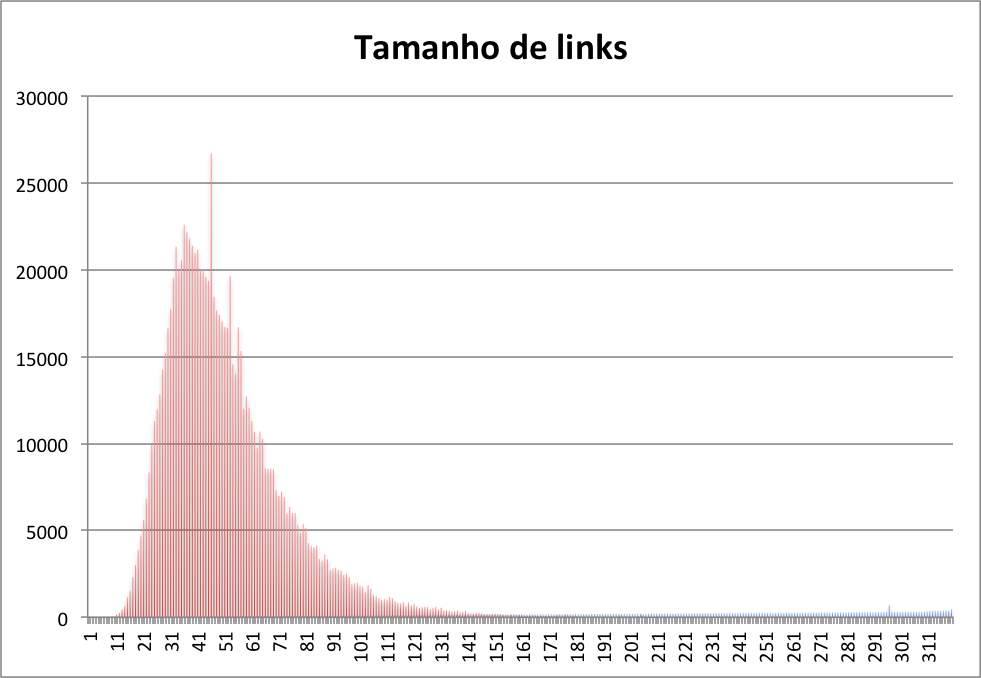
\includegraphics[scale=0.5]{distribuicaolinks.png}
    \caption{Distribuição do Tamanho dos links}
    \label{pic:distlinks}
\end{figure}

A computação do \emph{pagerank} é feita pela função \texttt{computa\_info\_links}, a qual se 
encontra no arquivo \texttt{colecao.cpp} e na classe \texttt{Colecao}. No código a seguir existem 
dois laços principais, o primeiro computa uma matriz de \emph{inlinks} de cada página e o segundo 
computa o \emph{pagerank} propriamente dito. Vamos analisar a memória 
gasta nesta função de acordo com as estruturas principais:

  \begin{itemize}
      \item \texttt{back\_links}: Esta estrutura mapeia os \emph{outlinks} de \texttt{indice\_link} 
	  para identificadores inteiros que representam os links. Assim agora não temos mais o mapeamento 
	  link -> outlinks, mas sim identificador -> link. Esta estrutura consome aproximadamente 
	  ($945642\times20$$\times4bytes$) 72MB de memória.
      \item \texttt{pr}: Esta estrutura armazena o \emph{pagerank} das páginas da coleção. Considerando 
	  que um \texttt{double} tem tamanho de 8 bytes, então esta estrutura consumirá aproximadamente 
	  7.2 MB de memória. A estrutura \texttt{old\_pr} consome a mesma quantidade de memória.
  \end{itemize}

\lstinputlisting{pr.cpp}

%TODO: esquecendo algo aqui
Durante a execução de \texttt{computa\_info\_links} o consumo de memória também incluirá as estruturas 
a seguir:
   \begin{itemize}
       \item \texttt{vocabulario} e \texttt{vocabulario\_invertido}: Aproximadamente estas estruturas consomem 
	   $(20+4)$ $\times 945642$ bytes, que resulta em 25MB de memória, pois a memória alocada para as palavras em 
	   \texttt{vocabulario} é a mesma utilizada em \texttt{vocabulario\_invertido}.
   \end{itemize}


No total o novo índice acrescenta mais 289.8 MB de memória ao gasto original. A complexidade de 
se calcular o pagerank é realizada após percorrer as páginas, então \underline{adiciona-se} a complexidade 
original apenas o tempo que se percorre todos os $D$ documentos duas vezes, i.e., \BigO{2|D|}.

A análise feita acima considera apenas a lógica do algoritmo, contudo a aplicação da
biblioteca \texttt{oneurl} deve também ser levada em consideração. Ao olhar o código fonte da função 
\texttt{CNormalize}(Url.cc) existem várias computações 
cuja complexidade é \BigO{|u|}, onde $|u|$ é o tamanho de uma dada URL. Contudo existem 
algumas computações que podem utilizar a biblioteca \texttt{map} do C++. Assim acredito que 
no pior caso a complexidade de \texttt{CNormalize} é \BigO{|u|log|u|}. Supondo que esta computação 
executa $l$ (número médio de links por página) vezes por documento,  nesta fase do sistema 
a complexidade de tempo de \texttt{ler\_arvore\_dom} muda para 
 \BigO{|D|(|t||s|+|l||u|log|u|)} no pior caso, onde $|D|$ é o número de documentos  
 na coleção, na média o tamanho da árvore DOM tem $|t|$ nós e 
$|s|$ é o número médio de caracteres por documento.


\subsubsection{\emph{Ranking}}

%== Ranking ==

%como eh calculado wd? 

%como a implementacao do BM25 esta no codigo?

%como a implementacao do vetorial esta no codigo?

% e a combinacao dos dois?

A computação do \emph{ranking} é feito no arquivo \texttt{ranking.cpp}, o qual 
contém as seguintes classes: 
    \begin{itemize}
         \item  \texttt{Ranking}: Esta classe descreve métodos abstratos e métodos 
	     concretos. Os métodos abstratos são métodos que todas as classes de 
	     \emph{ranking} devem implementar de acordo com suas características 
	     particulares. Os métodos concretos implementados nesta classe são iguais 
	     para todas as classes de \emph{rankings} portanto não existe a necessidade 
	     de implementação pelas classes filhas.
	 \item \texttt{Vetorial}: Esta classe herda a classe \texttt{Ranking} e 
	     implementa o modelo Vetorial de \emph{ranking}\cite{Baeza1999}.
	 \item \texttt{BM25}: Esta classe herda a classe \texttt{Ranking} e 
	     implementa o modelo BM25 de \emph{ranking}\cite{Baeza1999}. Nesta 
	     fase foi implementada a normalização do BM25, que consiste apenas 
	     da divisão da pontuação  de cada documento pelo maior valor de pontuação 
	     computado.
	 \item\texttt{MIX}: Esta classe herda a classe \texttt{Ranking} e implementa 
	     a \emph{power mean}\cite{powermean} entre as pontuações do modelo Vetorial e 
	     modelo BM25.
     \end{itemize}

 Para computar os \emph{rankings} de maneira eficiente, a computação dos pesos de cada 
 documento são pré-computadas e armazenadas no arquivo \texttt{wd\_compacta.txt}. A criação 
 deste arquivo é controlada pela variável \texttt{constroi\_wd} no arquivo \texttt{pesquisa.cpp}. 
 Por padrão esta variável está com valor \texttt{false}. No entanto, na primeira execução 
 do sistema esta variável deve estar inicializada com valor \texttt{true} para que este 
 arquivo seja criado. A criação deste arquivo percorre todo arquivo de índice e 
 vai armazenando as frequências dos termos para cada documento. A função que 
 executa esta computação está em \texttt{ranking.cpp} e se chama 
 \texttt{escreve\_wd}. O pseudo-código que computa o peso $wd(i)$ do i-ésimo documento 
 está descrito como a seguir.



\section{Resultados e Avaliação}

%diferenca no tempo de indexacao, vocabulario e no. de triplas

% e tempo do calculo do pagerank?

%diferenca no tamanho do vocabulario, (indice?)

%Explicitar tamanho de constantes: ITER_PR, p (do power mean)

%tempo que demora para carregar o vocabulario

Como já foi mencionado anteriormente a indexação nos trabalhos passados considerou o 
conteúdo do texto âncora. Contudo para fazer uma comparação mais justa gerei o índice 
novamente com e sem texto âncora. A Tabela \ref{tbl:indexnum} descreve a diferença no 
tempo da indexação (total) 
e do tamanho do vocabulário destas duas abordagens.

\begin{table}[H]
    \centering
    \begin{tabular}{l|c|c|c} \hline
	Abordagem        & \#triplas & \#palavras & Tempo (s) \\ \hline \hline
	Sem Texto Âncora &  381884617& 6154031    & 9200.66  \\
	Com texto Âncora &  539785346& 8200561    & 11902.95    \\ \hline
    \end{tabular}
    \caption{Tabela mostrando o desempenho das Abordagens de Indexação}
    \label{tbl:indexnum}
\end{table}

Como era de se esperar todos os valores de \#triplas, de \#palavras e de Tempo aumentaram 
com a inclusão de texto âncora no índice. A explicação óbvia é que o texto âncora possui 
palavras que antes não eram indexadas e que indexando, geram novas triplas no índice. Mais palavras 
e triplas também exige mais tempo para ordenação e processamento das mesmas, portanto 
é natural que o tempo de execução da indexação aumente.

Ambas abordagens da Tabela \ref{tbl:indexnum} já incluem a computação do \emph{pagerank}. O 
cálculo do \emph{pagerank} do meu sistema considera 50 iterações para chegar no valor final. 
De acordo Page et. al ~\cite{page1999pagerank} a partir de 50 iterações o \emph{pagerank} 
converge. O valor da iterações pode ser modificado no arquivo \texttt{util.h} através da 
constante \texttt{ITER\_PR}. Para computar o \emph{pagerank} também foi considerado 
o \emph{dumping factor}, que é a probabilidade do usuário, de chegar em uma página $u$ 
a partir de algum de seus \emph{links} de entrada. O valor desta constante foi inicializado 
como $0.85$. Contudo o valor do \emph{dumping factor} pode ser modificado através da constante
\texttt{D\_FACTOR} no arquivo \texttt{util.h}.

\section{Conclusão}

\appendix

\section{Manual do Sistema}

Três etapas são necessárias para a execução da pesquisa: configuração, 
compilação e a execução do sistema. As próximas subseções descrevem 
como fazer estas etapas.

\subsection{Configurar}


Para a construção do pagerank foi necessárias algumas poucas modificações 
na construção do índice. Portanto antes de executar a pesquisa é necessária 
a execução da construção do índice. Estas modificações podem ser relativas 
a arquivos criados ou podem ser relativos a lógica do algoritmo de 
indexação.

As modificações implementadas no índice relativas a arquivos são:

\begin{enumerate}
   \item Criação de um arquivo que armazena informações de cada documento, a saber: 
tamanho em palavras e pagerank. Este arquivo por padrão se chama info\_arquivos.txt;
   \item Ao vocabulário foi adicionada a frequência do termo na coleção.
\end{enumerate}

As modificações relativas a implementação estão relacionadas com a construção 
do pagerank. Como a catalogação de links e posteriormente o cálculo do pagerank.  
Para a catalogação de links pensei em normalizar as URLs a fim de obter um 
resultado com mais acurácia. A normalização de links foi feita utilizando 
a biblioteca oneurl\footnote{\url{https://github.com/nuoline/oneurl}}. Logo 
no pacote deste trabalho existe uma pasta com o código fonte do oneurl. 
A compilação da biblioteca oneurl exige a instalação do icu4c, cujo download 
pode ser feito no site \url{http://site.icu-project.org/download}. No ambiente linux e 
MacOSX é possível fazer a instalação do icu4c via gerenciador de pacotes. A 
compilação do oneurl será abordado na próxima seção.

O sistema proposto é compilado através de Makefile. A primeira parte da configuração 
deve ser feita no Makefile do diretório principal do sistema. No início do Makefile 
existe um conjunto de variáveis que deve ser modificado conforme os diretórios 
do usuário. Segue uma lista de tais variáveis e a explicação de cada uma.

   \begin{itemize}
      \item  ricode: Diretório onde estão armazenados os códigos objetos da biblioteca CollectionReader;
      \item  urlcode: Diretório com os arquivos de cabeçalho da biblioteca oneurl;
      \item ridata: Diretório onde se encontra o arquivo com a lista de documentos a serem indexados;
      \item  riindex: nome do arquivo que contém os links dos documentos a serem processados para o índice;
  \end{itemize}

A segunda parte da configuração se encontra dentro no início do arquivo colecao.cpp. A configuração 
em colecao.cpp engloba os nomes dos arquivos a serem gerados. Seguem as declarações 
das variáveis como no código fonte.

    \begin{itemize}
      \item  \texttt{const string Colecao::nome\_arquivo\_indice="index\_compacta.bin";}
      \item \texttt{const string Colecao::nome\_arquivo\_vocabulario="voc\_compacta.txt";}
      \item  \texttt{const string Colecao::nome\_info\_arquivos="info\_arquivos.txt";}
     \end{itemize}

A terceira parte da configuração se encontra no início do arquivo pesquisa.cpp e assim como 
a segunda parte da configuração armazena os nomes dos arquivos a serem gerados ou a serem lidos.
Seguem as declarações das variáveis como no código fonte.
 
   \begin{itemize}
      \item \texttt{const string Pesquisa::nome\_arquivo\_vocabulario = "voc\_compacta.txt";}
      \item \texttt{ const string Pesquisa::nome\_arquivo\_indice = "index\_compacta.bin";}
      \item  \texttt{const string Pesquisa::nome\_info\_arquivos = "info\_arquivos.txt";} 
      \item \texttt{const string Pesquisa::nome\_dir\_saida = "saida/"; //guarda resultados da pesquisa}
    \end{itemize}
%TODO: escolha do ranking
    A quarta parte da configuração é a escolha do 
    %TODO: como configurar para gerar o arquivo de wd (quanto tempo levou para gerar?)
\subsection{Compilar}

Caso a configuração tenha sido feita de forma correta a compilação do sistema 
segue como próximo passo. As subetapas da compilação da compilação são: compilação do oneurl, 
compilação do índice e compilação da pesquisa.

\subsubsection{Oneurl}

A compilação do oneurl é feita através da sequência de comandos a seguir:

~

\texttt{cd oneurl-master/ \&\& make \&\& cd ..}

~

Caso aconteça algum problema é possível que esteja relacionada com a biblioteca icu4c, pois 
o pacote do oneurl abrange a biblioteca icu4c já compilada. Isso não é recomendado visto que 
a instalação pode ocorrer em uma arquitetura diferente da arquitetura onde a icu4c foi 
compilada. Nesta situação basta modificar o Makefile da pasta oneurl-master para 
apontar para o icu4c que foi compilado nativamente em sua máquina.

\subsubsection{Índice}

A compilação do índice é feita através do comando: 

~

\texttt{make index}

~

Assumindo que os código objetos do CollectionReader já existam, caso contrário 
é necessário executar make ziplib antes de make index.

\subsubsection{Pesquisa}

A compilação da pesquisa é feita através do comando:

~

\texttt{make pesquisa}

\subsection{Testar}

\bibliographystyle{plain}
\bibliography{relatorio}
 
\end{document}


